\documentclass[11pt]{article}
\usepackage[margin=1in]{geometry}
\usepackage{graphicx}
\usepackage{booktabs}
\usepackage{caption}
\usepackage{subcaption}
\usepackage{hyperref}
\usepackage[T1]{fontenc}
\usepackage{newunicodechar}
\newunicodechar{⊥}{\ensuremath{\perp}}
\newunicodechar{α}{\ensuremath{\alpha}}
\newunicodechar{·}{--}
\graphicspath{{../../results/chronoberg_clever_cov/}{../../results/hf_block_aware/}}
\title{Block-aware $\pi$ weights on labeled Hugging Face datasets}
\author{CFPerm prototype}
\date{}
\begin{document}
\maketitle
\noindent Analyst-defined feature-blocks and Stage-1 consensus $\pi$ guide Stage-2 training: 
$\pi$-weighted RF (column replicates so $\mathtt{max\_features}$ samples $p_j\propto\pi_m/|B_m|$), 
a linear opinion pool $\sum_m\pi_m\hat e_m$, and $X{+}Z$ stacking. 
$Y$ is the dataset label; $W$ is the batch/domain used for FSDS.

\section{Overview dashboard}
\begin{figure}[h]
\centering
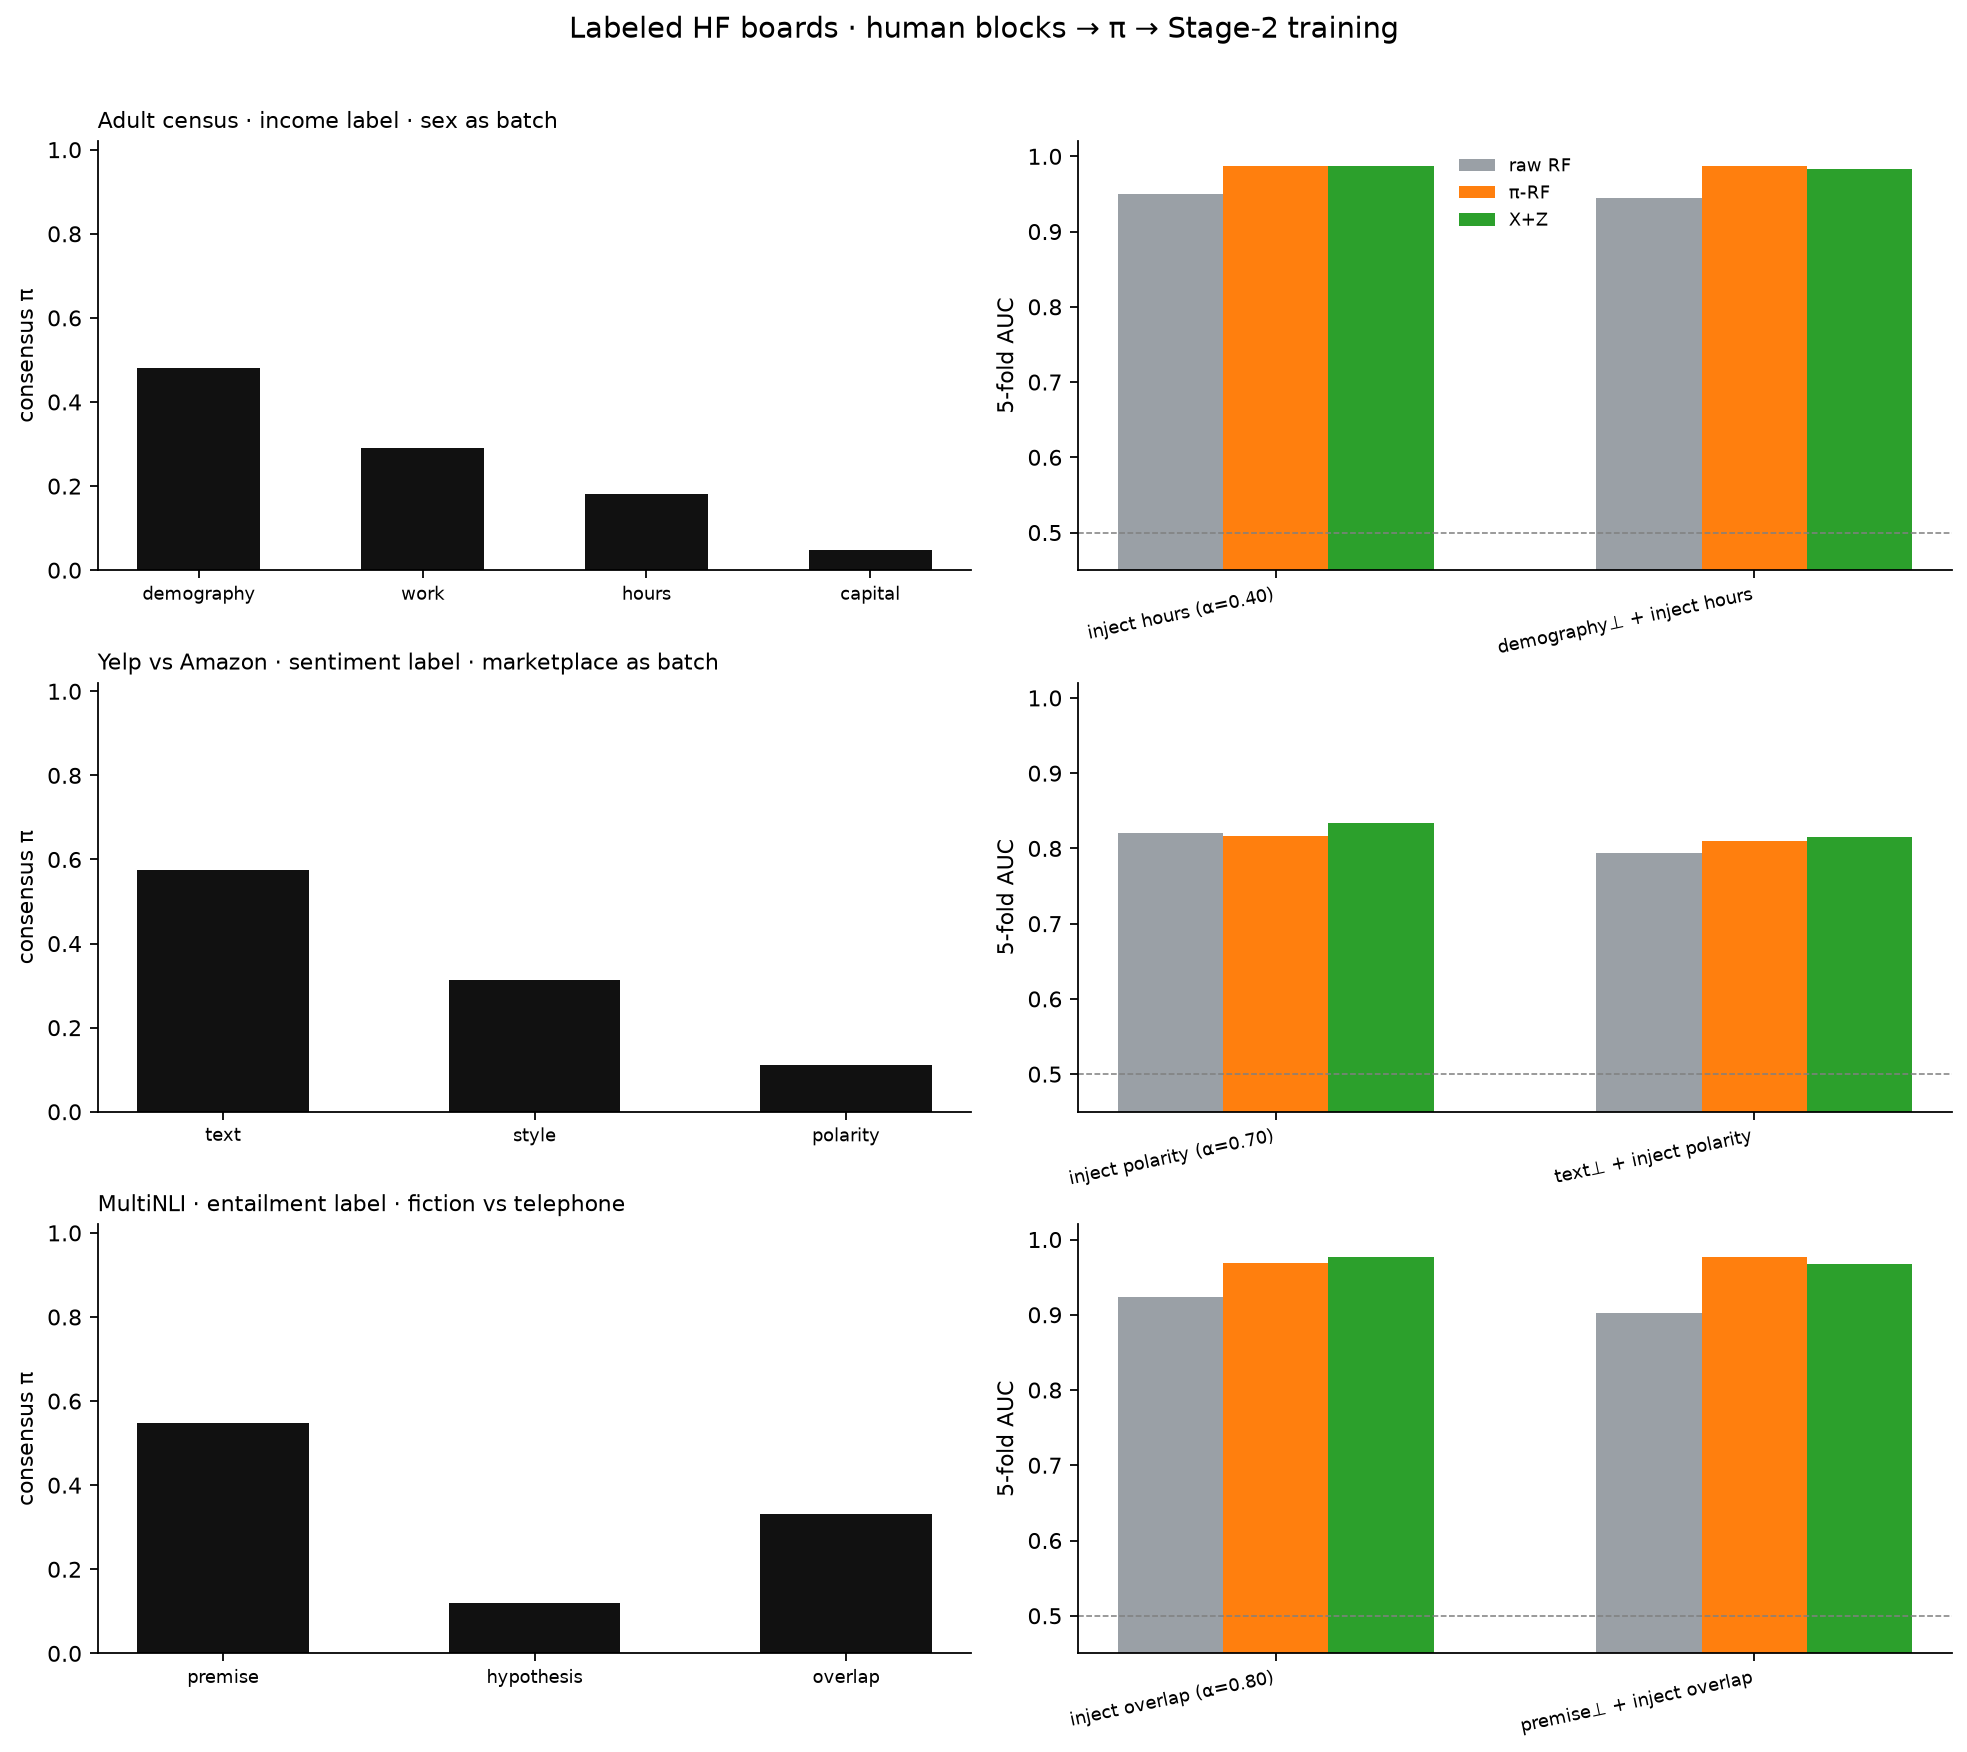
\includegraphics[width=\textwidth]{dashboard.png}
\caption{Each row is one labeled Hugging Face board. Left: Stage-1 consensus $\pi$ over human blocks. 
Right: 5-fold domain AUC on concentrated inject-GT (raw RF vs $\pi$-weighted RF vs $X{+}Z$).}
\label{fig:hf-dashboard}
\end{figure}

\section{Chronoberg (temporal text, VAD blocks)}
Temporal batch $W=1750$ vs.\ $1950$ on \texttt{spaul25/Chronoberg}; modalities hashed text / valence / arousal / dominance.
\begin{figure}[h]
\centering
\begin{subfigure}[t]{0.48\textwidth}
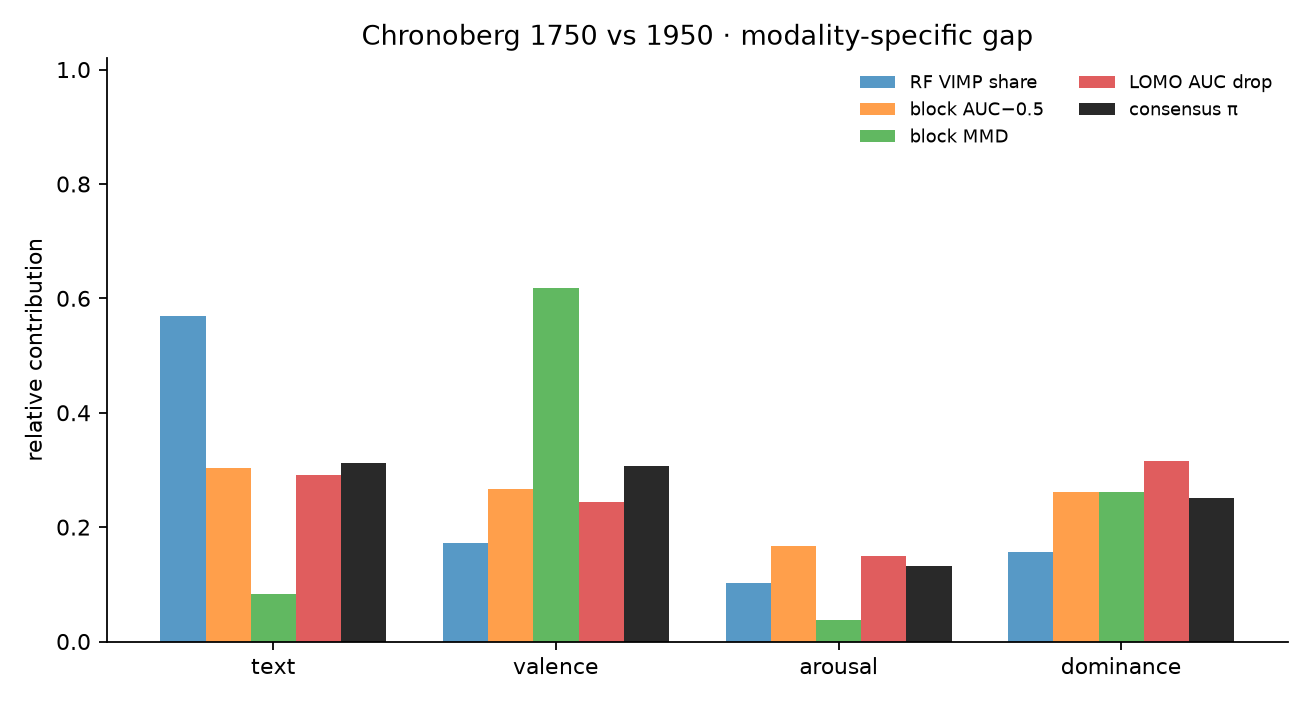
\includegraphics[width=\linewidth]{chronoberg_modality_gap_shares.png}
\caption{Stage-1 gap shares.}
\end{subfigure}\hfill
\begin{subfigure}[t]{0.48\textwidth}
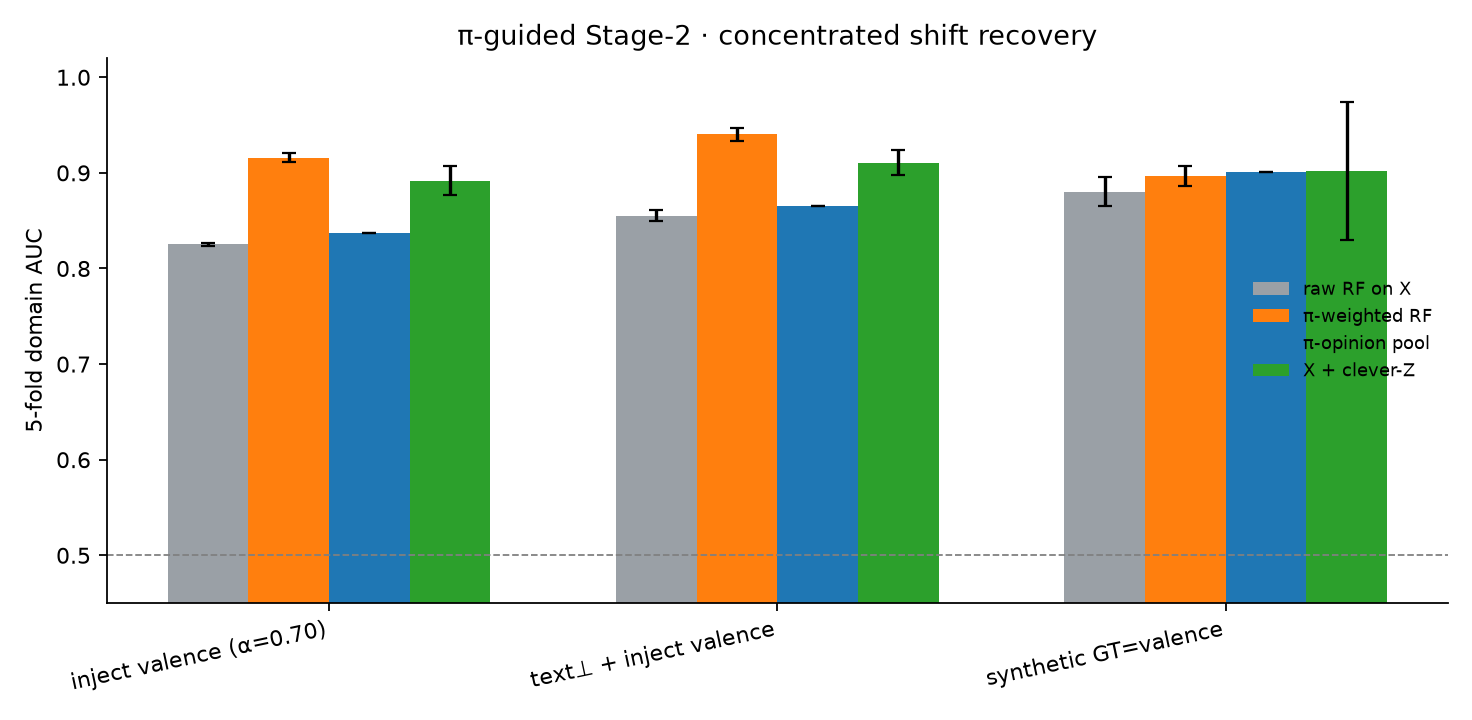
\includegraphics[width=\linewidth]{chronoberg_clever_vs_raw_auc.png}
\caption{$\pi$-guided Stage-2 GT board.}
\end{subfigure}
\caption{Chronoberg 1750 vs.\ 1950. Observational shift is diffuse; wins are on concentrated valence inject.}
\label{fig:chrono}
\end{figure}
\begin{figure}[h]
\centering
\begin{subfigure}[t]{0.48\textwidth}
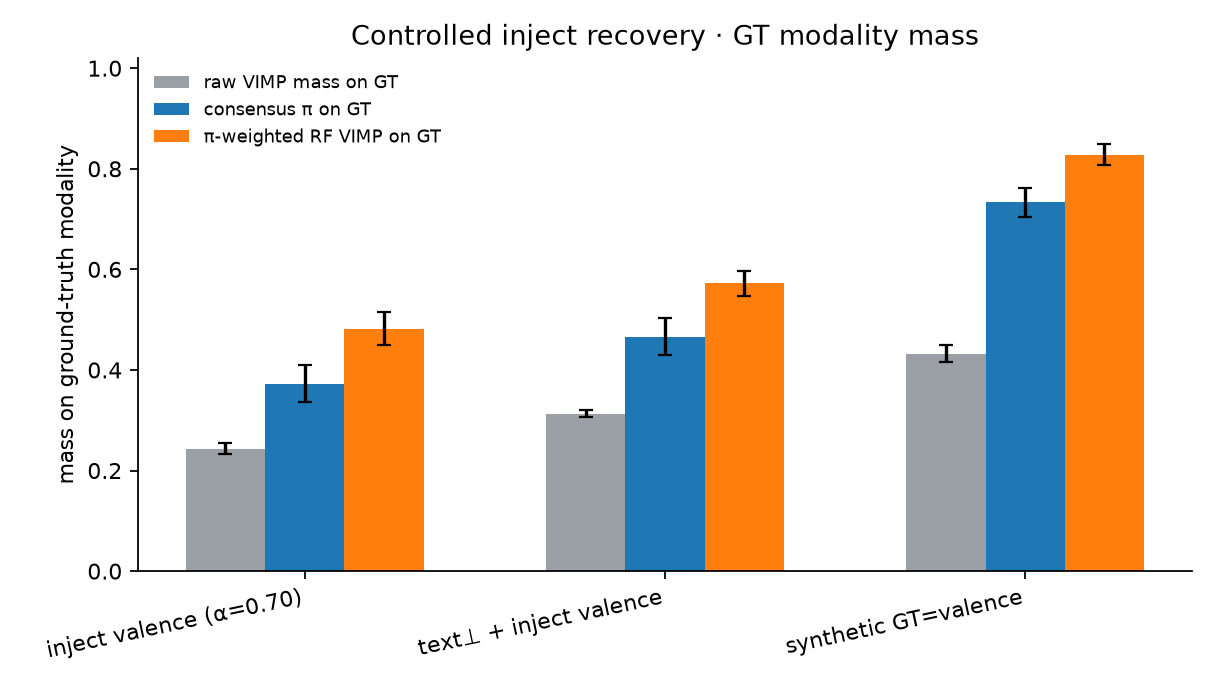
\includegraphics[width=\linewidth]{chronoberg_inject_recovery.png}
\caption{GT mass: raw VIMP vs $\pi$ vs $\pi$-RF.}
\end{subfigure}\hfill
\begin{subfigure}[t]{0.48\textwidth}
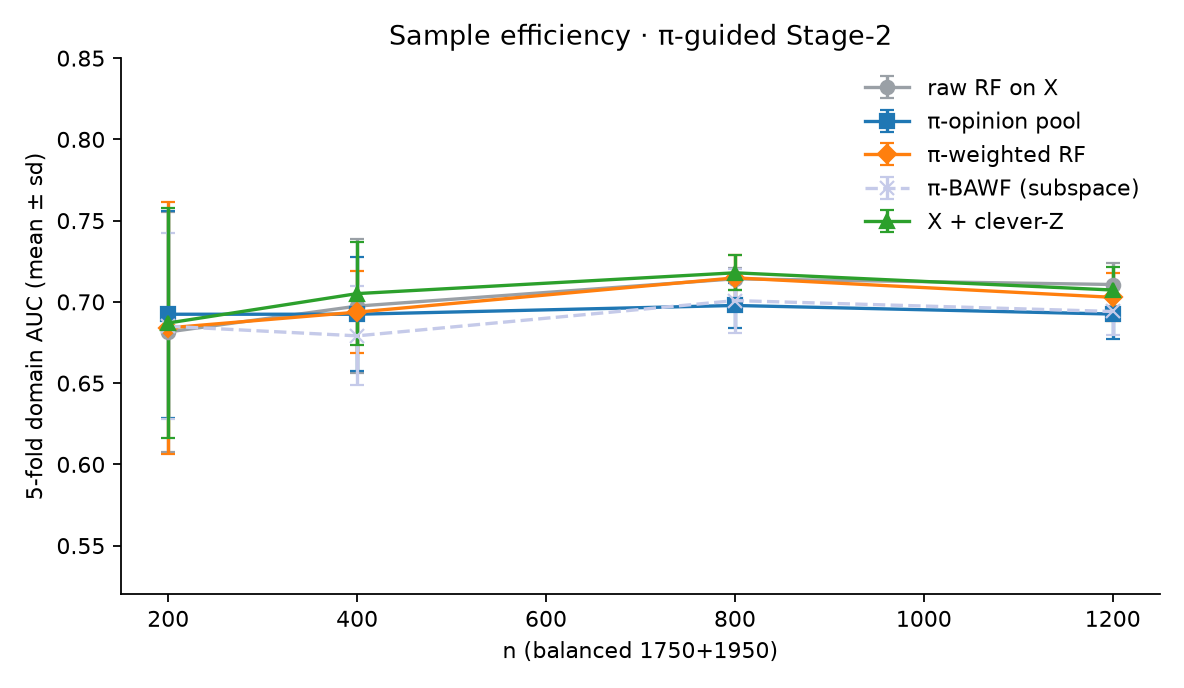
\includegraphics[width=\linewidth]{chronoberg_sample_efficiency.png}
\caption{Sample efficiency on the observational split.}
\end{subfigure}
\caption{Chronoberg localization and $n$-scaling.}
\end{figure}

\begin{table}[t]
\centering
\small
\caption{Chronoberg 1750 vs.\ 1950: modality-specific gap shares and clever-covariate FSDS.}
\begin{tabular}{lcccc}
\toprule
Decomposition & text & valence & arousal & dominance \\
\midrule
RF VIMP & 0.492 & 0.219 & 0.097 & 0.192 \\
block AUC & 0.419 & 0.293 & 0.036 & 0.252 \\
block MMD & 0.014 & 0.579 & 0.000 & 0.407 \\
LOMO drop & 0.243 & 0.349 & 0.191 & 0.217 \\
consensus $\pi$ & 0.282 & 0.343 & 0.109 & 0.266 \\
\bottomrule
\end{tabular}
\end{table}

\begin{table}[t]
\centering
\small
\caption{Raw $X$ vs.\ compact clever covariates $Z$ (instance $\pi_m(x)$ + logit $\hat e_m$).}
\begin{tabular}{lcccc}
\toprule
Setting & AUC raw $X$ & AUC clever-$Z$ & AUC $X{+}Z$ & $\Delta_{X+Z}$ \\
\midrule
observational 1750/1950 & 0.739 & 0.692 & 0.690 & -0.049 \\
CD: Y=valence, X=text+A+D & 0.710 & 0.637 & 0.638 & -0.072 \\
inject valence (α=0.95) & 0.859 & 0.816 & 0.875 & +0.015 \\
inject text (α=0.75) & 0.999 & 1.000 & 1.000 & +0.001 \\
text-shuffled + inject valence & 0.888 & 0.816 & 0.913 & +0.025 \\
synthetic GT=valence & 0.770 & 0.879 & 0.944 & +0.175 \\
\bottomrule
\end{tabular}
\end{table}



\section{Adult census  --  income label  --  sex as batch}
\noindent Dataset: \texttt{scikit-learn/adult-census-income}. 
Label $Y$: income >50K. W = sex (Female vs Male); relationship dropped (Husband/Wife leak). 
$n_0=800$, $n_1=800$.
\begin{figure}[h]
\centering
\begin{subfigure}[t]{0.48\textwidth}
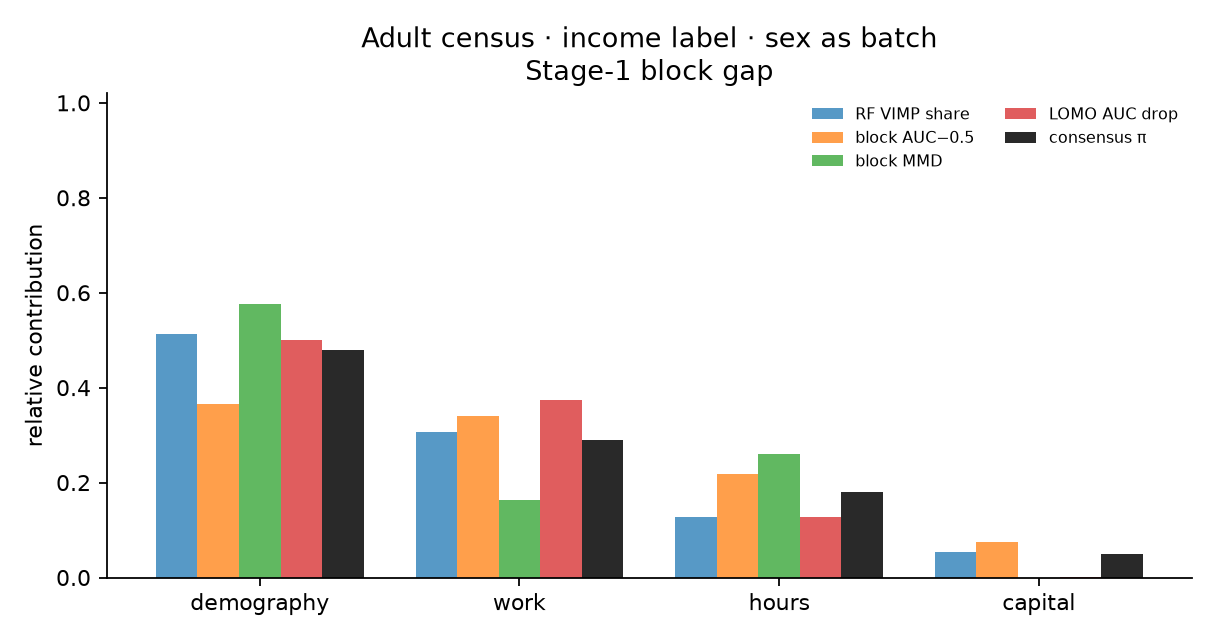
\includegraphics[width=\linewidth]{adult/adult_gap_shares.png}
\caption{Stage-1 block gap.}
\end{subfigure}\hfill
\begin{subfigure}[t]{0.48\textwidth}
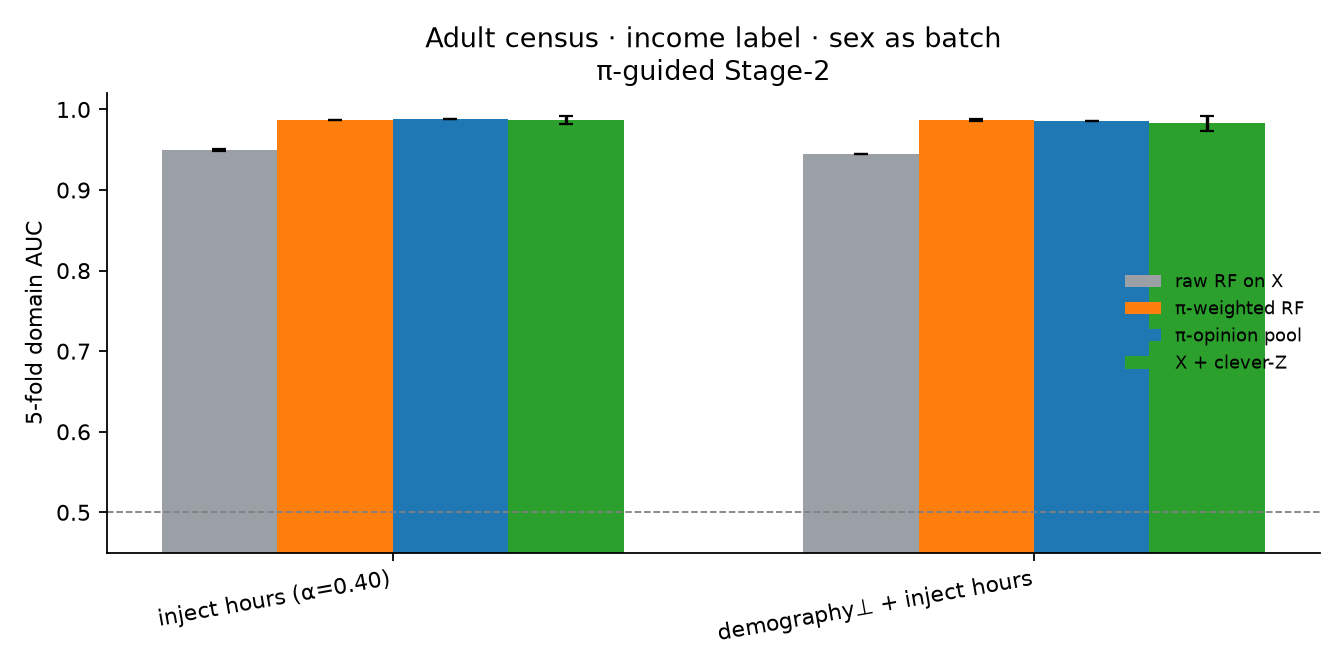
\includegraphics[width=\linewidth]{adult/adult_stage2_auc.png}
\caption{Stage-2 domain AUC.}
\end{subfigure}
\caption{Adult census  --  income label  --  sex as batch: human blocks and $\pi$-guided training. Observational rows can be diffuse; inject-GT is the concentrated-shift check.}
\label{fig:adult}
\end{figure}
\begin{figure}[h]
\centering
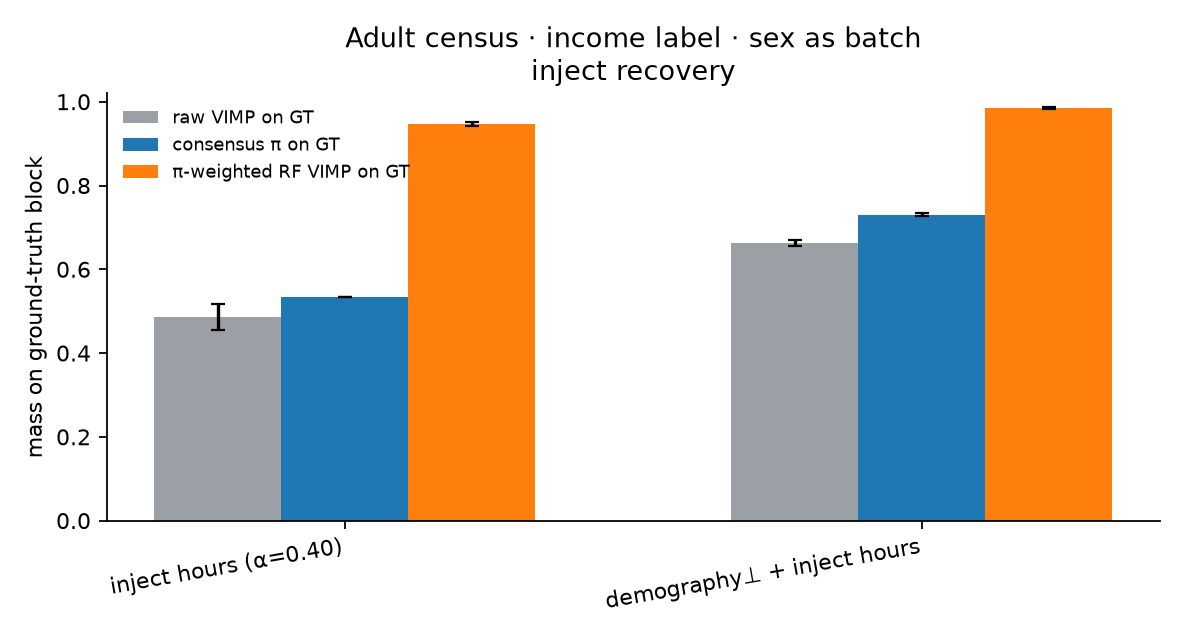
\includegraphics[width=0.72\textwidth]{adult/adult_inject_recovery.png}
\caption{Adult census  --  income label  --  sex as batch: mass on the ground-truth block after inject. $\pi$-weighted RF should concentrate relative to raw VIMP.}
\end{figure}

\begin{table}[t]
\centering
\small
\caption{Adult census  --  income label  --  sex as batch: Stage-1 block shares. $Y$=income >50K; W = sex (Female vs Male); relationship dropped (Husband/Wife leak).}
\begin{tabular}{lcccc}
\toprule
Decomposition & demography & work & hours & capital \\
\midrule
RF VIMP & 0.514 & 0.306 & 0.128 & 0.053 \\
block AUC & 0.366 & 0.341 & 0.218 & 0.075 \\
block MMD & 0.576 & 0.164 & 0.261 & 0.000 \\
LOMO drop & 0.499 & 0.373 & 0.127 & 0.000 \\
consensus $\pi$ & 0.480 & 0.290 & 0.181 & 0.049 \\
\bottomrule
\end{tabular}
\end{table}

\begin{table}[t]
\centering
\small
\caption{Adult census  --  income label  --  sex as batch: Stage-2 $\pi$-guided training (5-fold CV AUC).}
\begin{tabular}{lcccccc}
\toprule
Setting & raw RF & $\pi$-RF & pool & $X{+}Z$ & $\Delta_{\pi\mathrm{-RF}}$ & $\pi$-RF on GT \\
\midrule
observational & 0.855 & 0.849 & 0.845 & 0.857 & -0.006 & --- \\
inject hours ($\alpha$=0.40) & 0.950 & 0.987 & 0.988 & 0.987 & +0.037 & 0.947 \\
demography$\perp$ + inject hours & 0.945 & 0.987 & 0.986 & 0.983 & +0.042 & 0.984 \\
\bottomrule
\end{tabular}
\end{table}



\section{Yelp vs Amazon  --  sentiment label  --  marketplace as batch}
\noindent Dataset: \texttt{fancyzhx/yelp\_polarity vs fancyzhx/amazon\_polarity}. 
Label $Y$: binary sentiment. W = marketplace (Yelp vs Amazon); reviews truncated to 50 tokens. 
$n_0=800$, $n_1=800$.
\begin{figure}[h]
\centering
\begin{subfigure}[t]{0.48\textwidth}
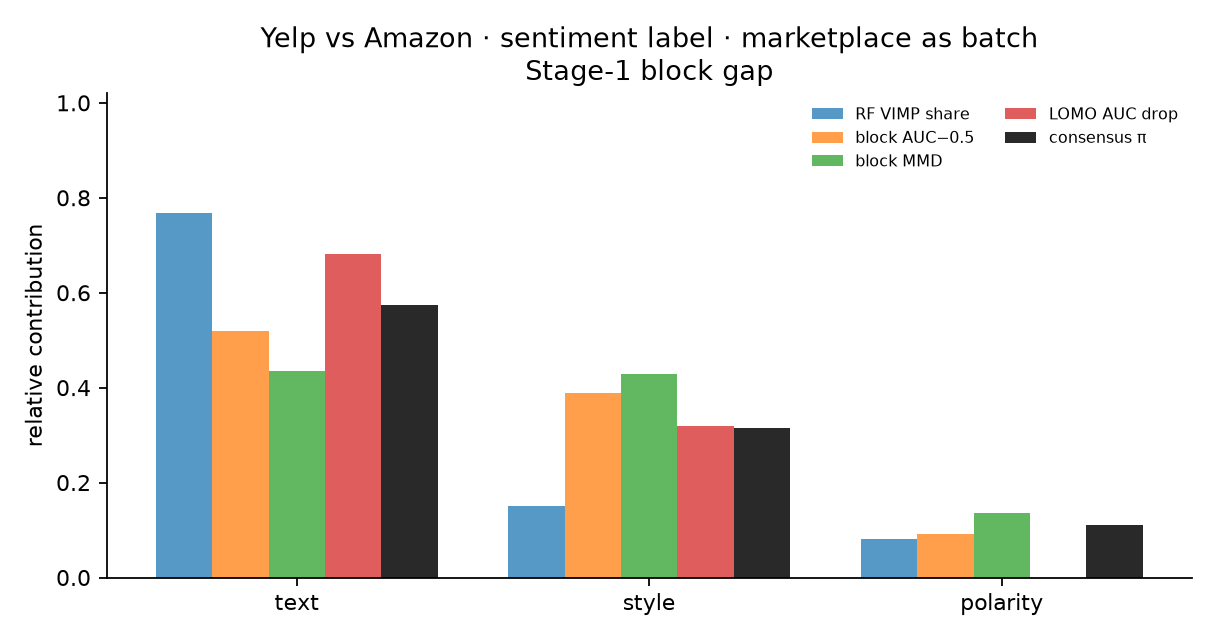
\includegraphics[width=\linewidth]{yelp_amazon/yelp_amazon_gap_shares.png}
\caption{Stage-1 block gap.}
\end{subfigure}\hfill
\begin{subfigure}[t]{0.48\textwidth}
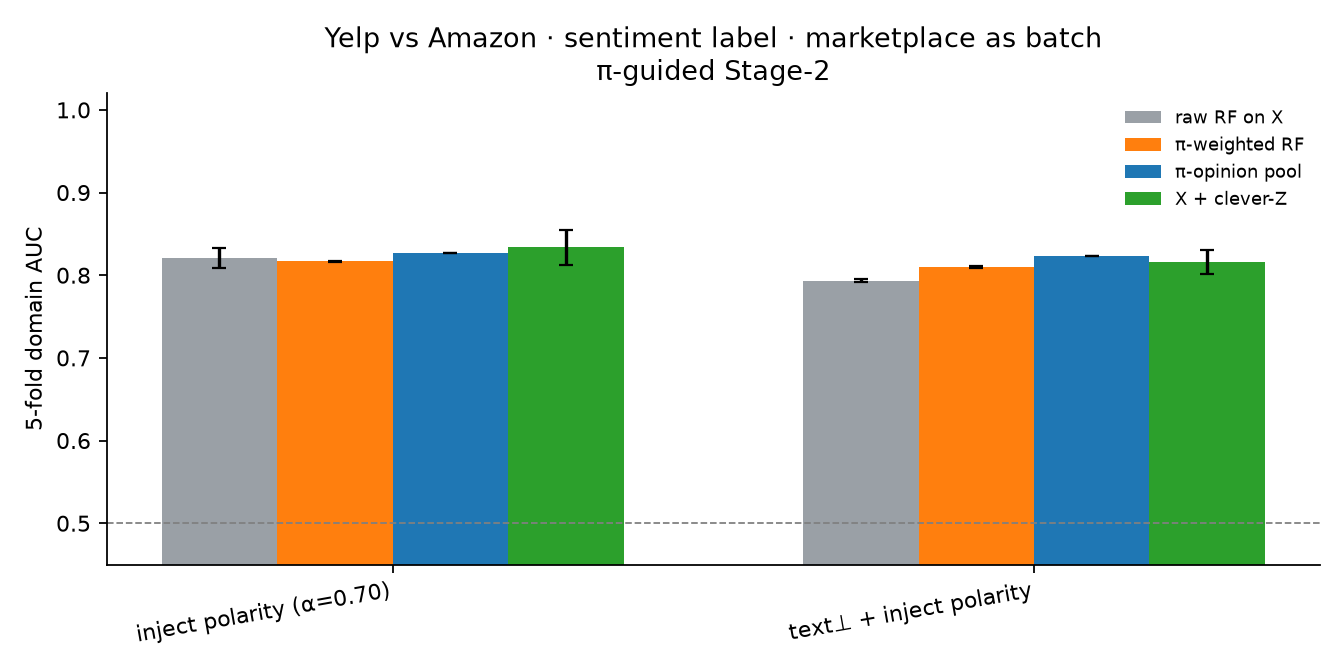
\includegraphics[width=\linewidth]{yelp_amazon/yelp_amazon_stage2_auc.png}
\caption{Stage-2 domain AUC.}
\end{subfigure}
\caption{Yelp vs Amazon  --  sentiment label  --  marketplace as batch: human blocks and $\pi$-guided training. Observational rows can be diffuse; inject-GT is the concentrated-shift check.}
\label{fig:yelp_amazon}
\end{figure}
\begin{figure}[h]
\centering
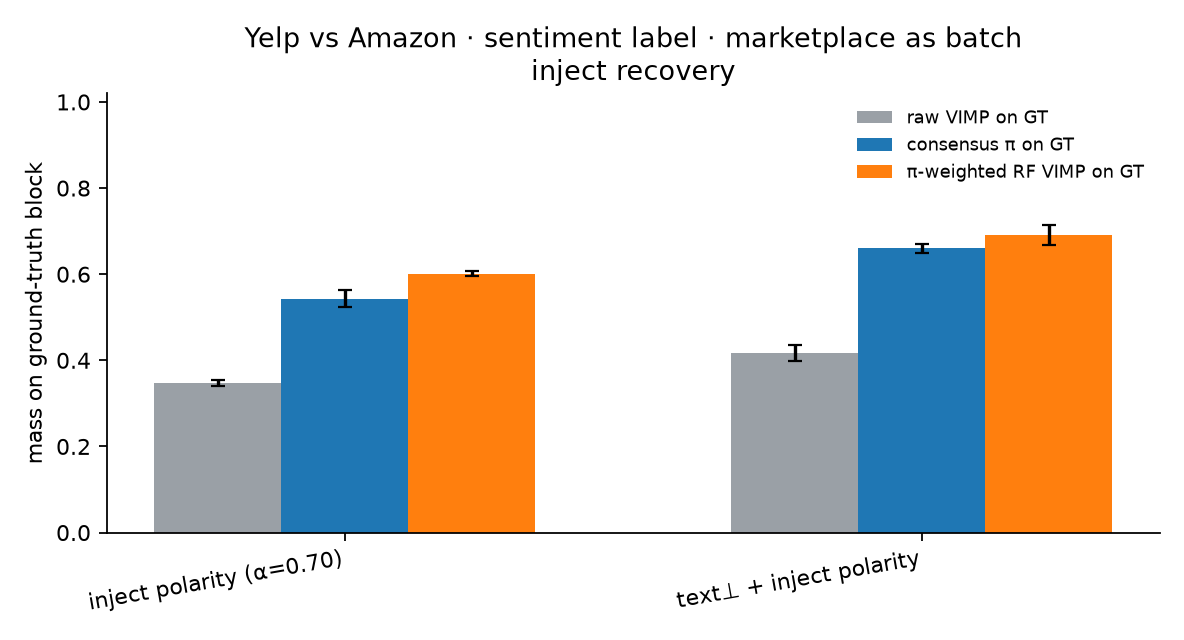
\includegraphics[width=0.72\textwidth]{yelp_amazon/yelp_amazon_inject_recovery.png}
\caption{Yelp vs Amazon  --  sentiment label  --  marketplace as batch: mass on the ground-truth block after inject. $\pi$-weighted RF should concentrate relative to raw VIMP.}
\end{figure}

\begin{table}[t]
\centering
\small
\caption{Yelp vs Amazon  --  sentiment label  --  marketplace as batch: Stage-1 block shares. $Y$=binary sentiment; W = marketplace (Yelp vs Amazon); reviews truncated to 50 tokens.}
\begin{tabular}{lccc}
\toprule
Decomposition & text & style & polarity \\
\midrule
RF VIMP & 0.767 & 0.151 & 0.082 \\
block AUC & 0.519 & 0.389 & 0.092 \\
block MMD & 0.435 & 0.429 & 0.136 \\
LOMO drop & 0.681 & 0.319 & 0.000 \\
consensus $\pi$ & 0.575 & 0.314 & 0.111 \\
\bottomrule
\end{tabular}
\end{table}

\begin{table}[t]
\centering
\small
\caption{Yelp vs Amazon  --  sentiment label  --  marketplace as batch: Stage-2 $\pi$-guided training (5-fold CV AUC).}
\begin{tabular}{lcccccc}
\toprule
Setting & raw RF & $\pi$-RF & pool & $X{+}Z$ & $\Delta_{\pi\mathrm{-RF}}$ & $\pi$-RF on GT \\
\midrule
observational & 0.728 & 0.725 & 0.729 & 0.727 & -0.003 & --- \\
inject polarity ($\alpha$=0.70) & 0.821 & 0.817 & 0.827 & 0.834 & -0.004 & 0.602 \\
text$\perp$ + inject polarity & 0.794 & 0.810 & 0.823 & 0.816 & +0.016 & 0.691 \\
\bottomrule
\end{tabular}
\end{table}



\section{MultiNLI  --  entailment label  --  fiction vs telephone}
\noindent Dataset: \texttt{nyu-mll/multi\_nli validation\_matched}. 
Label $Y$: entailment vs rest. W = genre (fiction vs telephone). 
$n_0=800$, $n_1=800$.
\begin{figure}[h]
\centering
\begin{subfigure}[t]{0.48\textwidth}
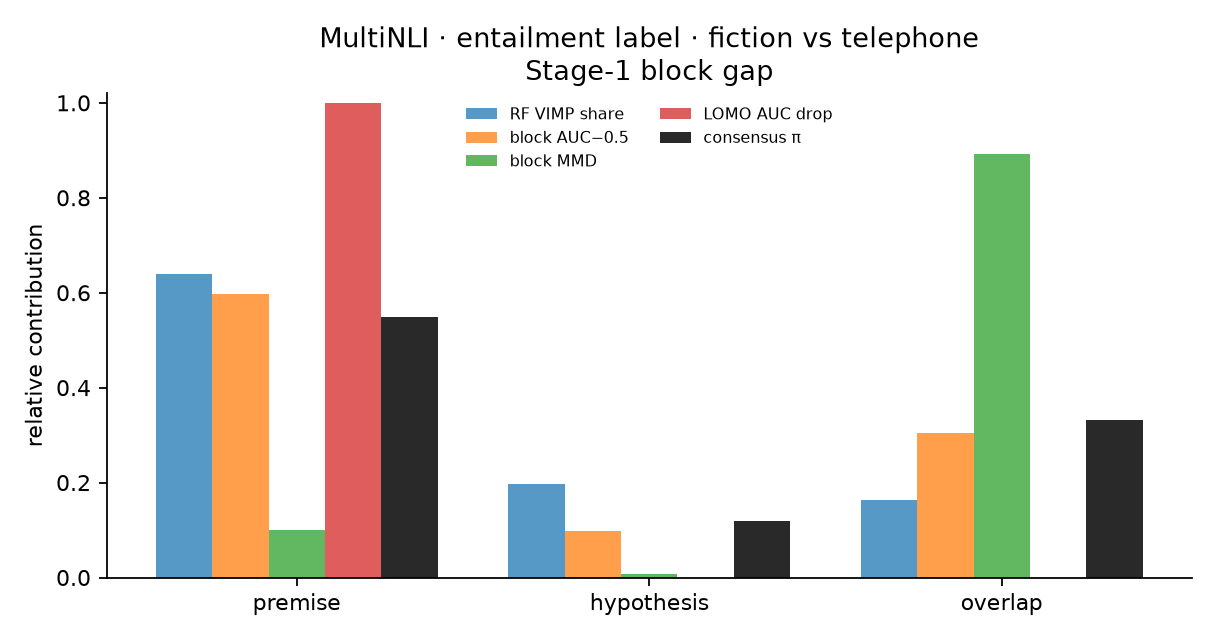
\includegraphics[width=\linewidth]{mnli/mnli_gap_shares.png}
\caption{Stage-1 block gap.}
\end{subfigure}\hfill
\begin{subfigure}[t]{0.48\textwidth}
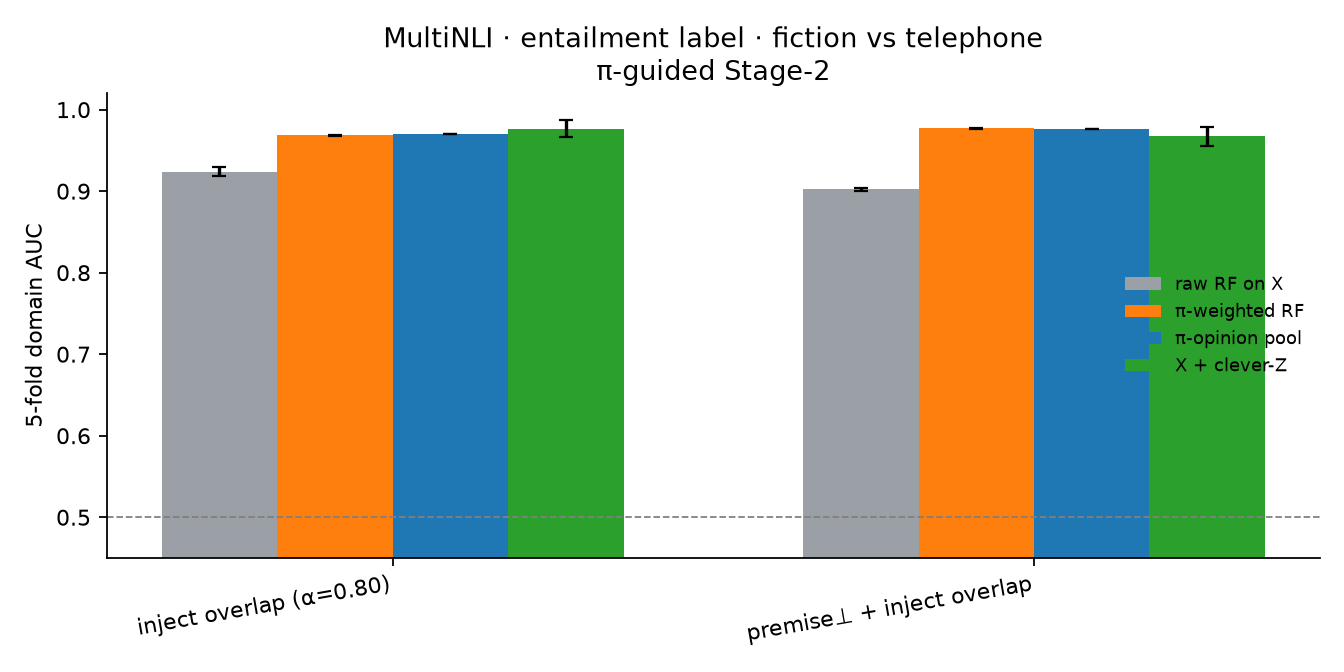
\includegraphics[width=\linewidth]{mnli/mnli_stage2_auc.png}
\caption{Stage-2 domain AUC.}
\end{subfigure}
\caption{MultiNLI  --  entailment label  --  fiction vs telephone: human blocks and $\pi$-guided training. Observational rows can be diffuse; inject-GT is the concentrated-shift check.}
\label{fig:mnli}
\end{figure}
\begin{figure}[h]
\centering
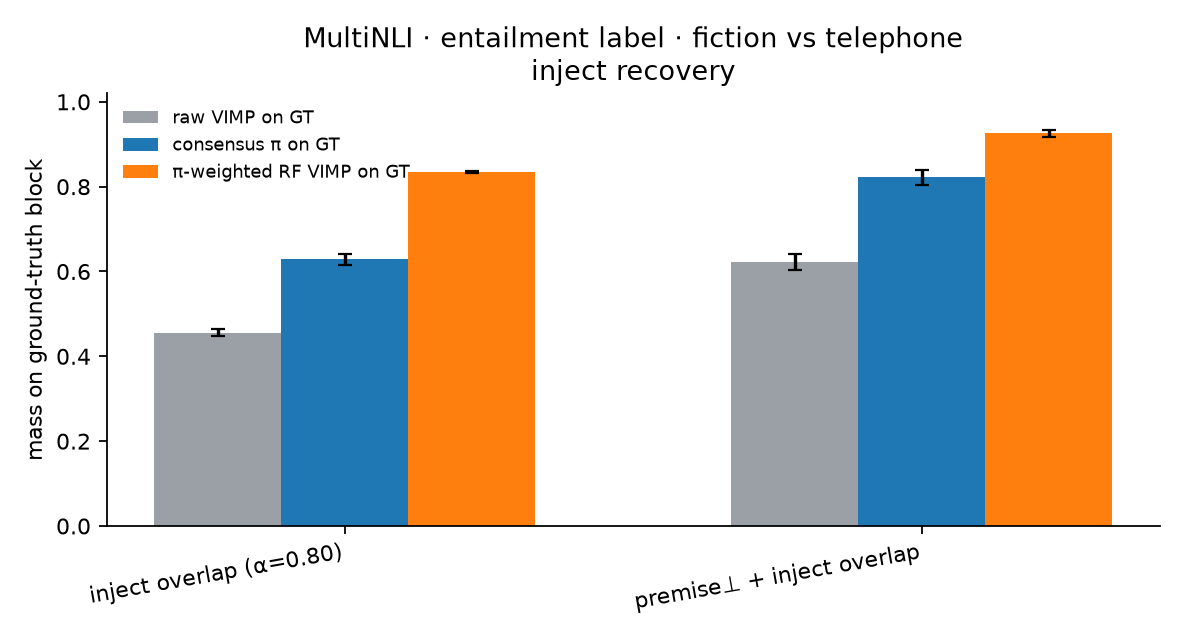
\includegraphics[width=0.72\textwidth]{mnli/mnli_inject_recovery.png}
\caption{MultiNLI  --  entailment label  --  fiction vs telephone: mass on the ground-truth block after inject. $\pi$-weighted RF should concentrate relative to raw VIMP.}
\end{figure}

\begin{table}[t]
\centering
\small
\caption{MultiNLI  --  entailment label  --  fiction vs telephone: Stage-1 block shares. $Y$=entailment vs rest; W = genre (fiction vs telephone).}
\begin{tabular}{lccc}
\toprule
Decomposition & premise & hypothesis & overlap \\
\midrule
RF VIMP & 0.640 & 0.196 & 0.163 \\
block AUC & 0.597 & 0.099 & 0.304 \\
block MMD & 0.101 & 0.008 & 0.891 \\
LOMO drop & 1.000 & 0.000 & 0.000 \\
consensus $\pi$ & 0.549 & 0.119 & 0.332 \\
\bottomrule
\end{tabular}
\end{table}

\begin{table}[t]
\centering
\small
\caption{MultiNLI  --  entailment label  --  fiction vs telephone: Stage-2 $\pi$-guided training (5-fold CV AUC).}
\begin{tabular}{lcccccc}
\toprule
Setting & raw RF & $\pi$-RF & pool & $X{+}Z$ & $\Delta_{\pi\mathrm{-RF}}$ & $\pi$-RF on GT \\
\midrule
observational & 0.836 & 0.818 & 0.848 & 0.875 & -0.018 & --- \\
inject overlap ($\alpha$=0.80) & 0.924 & 0.969 & 0.971 & 0.977 & +0.045 & 0.836 \\
premise$\perp$ + inject overlap & 0.902 & 0.977 & 0.977 & 0.967 & +0.075 & 0.926 \\
\bottomrule
\end{tabular}
\end{table}



\section{Cross-board notes}
\begin{itemize}
\item Trees ignore monotone column scaling; $\pi$ enters sklearn RF through column multiplicity.
\item Random-subspace BAWF is a different estimator class (not shown on these boards).
\item Adaptive group-logit can saturate on mean-shift inject; the RF analogue is the headline.
\item Observational Hugging Face shifts are often diffuse across blocks; the GT inject rows isolate whether $\pi$ guides training when the shift \emph{is} concentrated.
\end{itemize}
\end{document}

